\documentclass[english,compress]{beamer}

\usepackage[square,numbers]{natbib}
\usepackage{tcolorbox}
\usepackage{listings}
\newcommand{\cw}{\texttt} % to display a word as in code format
\setbeamertemplate{section page}
{
	\begin{centering}
	\begin{beamercolorbox}[sep=12pt,center]{part title}
	\usebeamerfont{section title}\insertsection\par
	\end{beamercolorbox}
	\end{centering}
}
\addtobeamertemplate{navigation symbols}{}{%
    \usebeamerfont{footline}%
    \usebeamercolor[fg]{footline}%
    \hspace{1em}%
    \insertframenumber/\inserttotalframenumber
}
\tcbuselibrary{listings}
\useoutertheme{split}
\useinnertheme{rectangles}
\usecolortheme{uiuc}
\logo{
\includegraphics[height=0.5cm]{uiuclogo.pdf}}
\AtBeginSection{\frame{\sectionpage}}

\title{SIAM: Getting Started with Git}
\subtitle{based on http://git-scm.com/book and slides by Bart Trojanowski}
\author{Andrew Reisner and Nathan Bowman}
\date{\today}

\begin{document}
\nocite{*}
\frame{\titlepage}
\frame{\frametitle{Table of Contents}\tableofcontents}

\section{Overview}
\frame
{
    \frametitle{Git}
    \begin{columns}
    \begin{column}{.5\textwidth}
        Git is a
        \begin{itemize}
            \item Free and Open Source
            \item Distributed
            \item Version Control System.
        \end{itemize}
    \end{column}
    \begin{column}{.5\textwidth}
        \begin{center}
            
\includegraphics[width=.7\textwidth]{figs/git-logo.png} 
        \end{center}
    \end{column}
    \end{columns}
}

\frame
{
    \frametitle{Version Control System}

        Preserve a clear, timely record of software evolution
            \begin{itemize}
                \item Record changes to files
                \item History can be recalled/inspected
            \end{itemize}
        Implications:
            \begin{itemize}
                \item Rollback changes
                \item Know what collaborators are working on
                \item Investigate changes when bugs emerge
                \item Find how and where a particular bug was fixed
            \end{itemize}
}

\section{Components}
\frame
{
    \frametitle{VCS Components (Working Tree)}

    \begin{itemize}
        \item Single checkout of one version of the project
        \item Directories
        \item Files
    \end{itemize}
    \begin{center}
        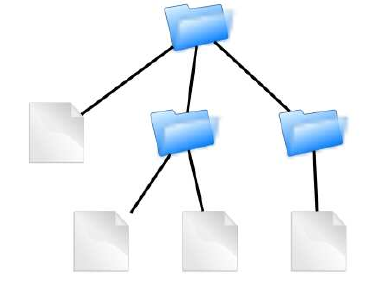
\includegraphics[height=.3\textwidth]{figs/working-tree.png}
    \end{center}
}

\frame
{
    \frametitle{VCS Components (Repository)}

    \begin{columns}
        \begin{column}{.5\textwidth}
    \begin{itemize}
        \item Files
        \item Commits
        \item Ancestry
    \end{itemize}
\end{column}
\begin{column}{.5\textwidth}
    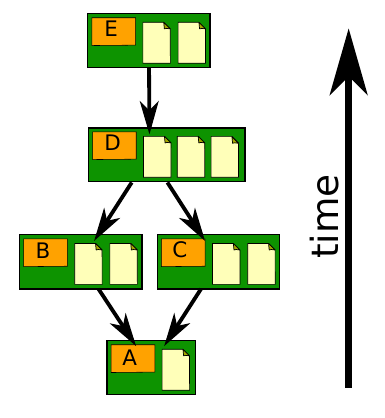
\includegraphics[width=.8\textwidth]{figs/repo.png}
\end{column}
\end{columns}
}

\frame
{
    \frametitle{VCS Components (References)}

    \begin{columns}
        \begin{column}{.5\textwidth}
    \begin{itemize}
        \item Tags
        \item Branches
    \end{itemize}
\end{column}
\begin{column}{.5\textwidth}
    \begin{itemize}
        \item HEAD
        \item Index (Staging area)
    \end{itemize}
\end{column}
\end{columns}
\begin{center}
    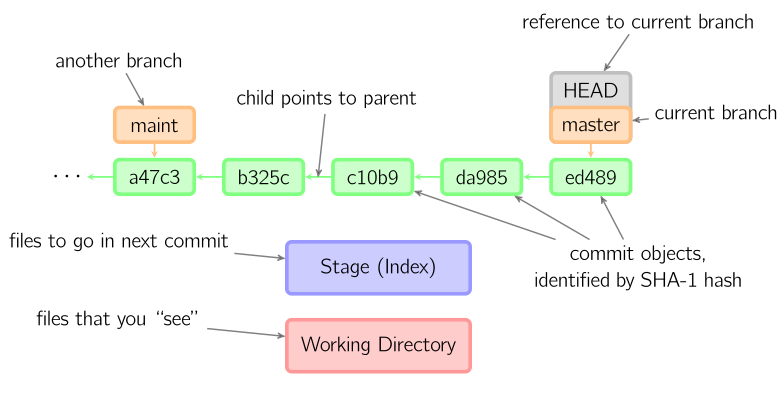
\includegraphics[width=\textwidth]{figs/visual-git.png}\cite{visual-git}
\end{center}
}

\frame
{
    \frametitle{VCS Components (Example Graph)}

	\begin{center}
		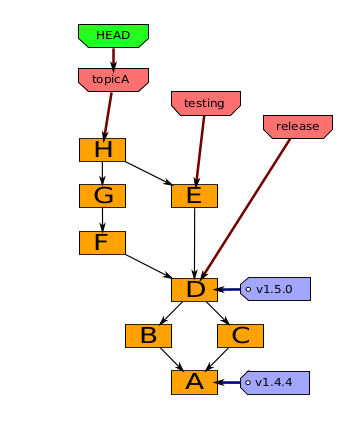
\includegraphics[height=.8\textheight]{figs/complicated-dag.png}
	\end{center}
}

\section{Operations}
\frame
{
    \frametitle{VCS Operations}
        \begin{columns}
            \begin{column}{.5\textwidth}
        Bootstrap
            \begin{itemize}
                \item \cw{init}
                \item \cw{clone}
            \end{itemize}
        Modify
        \begin{itemize}
            \item \cw{add}, delete (\cw{rm})
			\item rename (\cw{mv})
            \item \cw{commit}
        \end{itemize}
         Monitor Changes
        \begin{itemize}
            \item \cw{status}
            \item \cw{diff}
            \item \cw{log}
        \end{itemize}
   \end{column}
    \begin{column}{.5\textwidth}
        Undo
        \begin{itemize}
            \item \cw{checkout}
            \item \cw{reset}
        \end{itemize}
        Branch
        \begin{itemize}
            \item \cw{tag}
            \item \cw{branch}
            \item \cw{merge}
        \end{itemize}
        Share and Back Up
\begin{itemize}
    \item \cw{pull}, \cw{fetch}
    \item \cw{push}
\end{itemize}

    \end{column}
\end{columns}

}
\frame
{
    \begin{center}
        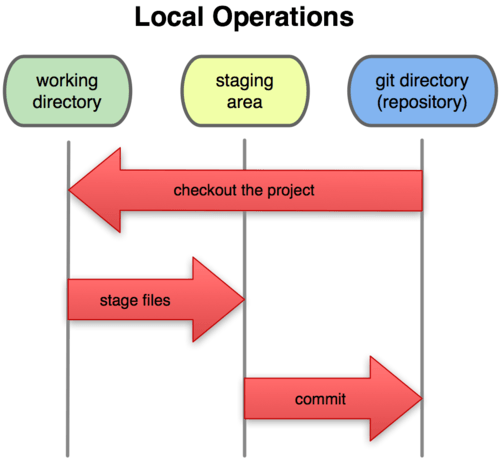
\includegraphics[width=.8\textwidth]{figs/sections.png}\cite{book}
    \end{center}
}

\subsection{Creating/Updating}
\begin{frame}[fragile]
    \frametitle{Bootstrapping}
    
    \verb|$ git init|
    \begin{itemize}
        \item creates .git directory and initializes the repository
    \end{itemize}
    \verb|$ git clone <URL>|
    \begin{itemize}
        \item replicates a remote repository
        \item checks out new working tree
        \item Git URLs
            \begin{itemize}
                \item /home/user/my-project.git
                \item http://github.com/user/my-project.git
                \item git://remote.server/my-project.git
                \item user@remote.server:my-project.git
                \item ssh://user@remote.server/~user/my-project.git
            \end{itemize}
    \end{itemize}
\end{frame}

\begin{frame}[fragile]
    \frametitle{Initializing Empty Repository}
    \begin{tcblisting}{listing only}
$ ls -a
. ..
$ git init
Initialized empty Git repository in /home/user/my-project/.git/
$ ls -a
. .. .git
$ ls
$
    \end{tcblisting}
\end{frame}

\begin{frame}[fragile]
    \frametitle{Staging}
    \verb|$ git add <path>|
    \begin{itemize}
        \item Adds contents of \verb|<path>| to index
        \item \verb|$ git add .|
    \end{itemize}
    
    \verb|$ git rm <file>|
    \begin{itemize}
        \item Removes files from working tree and index
    \end{itemize}

    \verb|$ git mv <source> <destination>|
    \begin{itemize}
        \item Moves or renames a file or directory
    \end{itemize}
\end{frame}

\begin{frame}[fragile]
    \frametitle{Adding our First File}
    \begin{tcblisting}{listing only}
$ echo 'Hi, my name is Andrew' > name_file.txt
$ git status
On branch master

Initial commit

Untracked files:
  (use "git add <file>..." to include in what will be committed)

	name_file.txt

nothing added to commit but untracked files present (use "git add" to track)
    \end{tcblisting}
\end{frame}

\begin{frame}[fragile]
    \frametitle{Adding our First File}
    \begin{tcblisting}{listing only}
$ git add name_file.txt
$ git status 
On branch master

Initial commit

Changes to be committed:
  (use "git rm --cached <file>..." to unstage)

	new file:   name_file.txt
    \end{tcblisting}
\end{frame}

\frame
{
    \begin{center}
        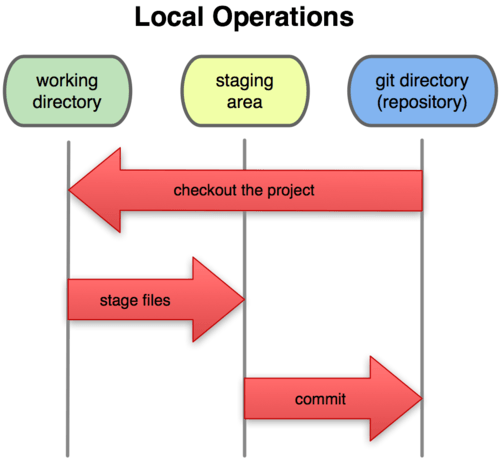
\includegraphics[width=.8\textwidth]{figs/sections.png}\cite{book}
    \end{center}
}

\begin{frame}[fragile]
    \frametitle{Committing}

    \verb|$ git commit -m <msg>|
    \begin{itemize}
        \item Creates a commit of staged items
        \item \verb|$ git commit -m "fixes issue #108"|
    \end{itemize}
\end{frame}

\begin{frame}[fragile]
    \frametitle{Creating our First Commit}
    \begin{tcblisting}{listing only}
$ git commit -m 'Add greeting'

*** Please tell me who you are.

Run

  git config --global user.email "you@example.com"
  git config --global user.name "Your Name"

to set your account's default identity.
Omit --global to set the identity only in this repository.

fatal: empty ident name (for <(null)>) not allowed
    \end{tcblisting}
\end{frame}

\begin{frame}[fragile]
    \frametitle{Creating our First Commit}
    \begin{tcblisting}{listing only}
$ git commit -m 'Add greeting'
[master (root-commit) dec6e96] Add greeting
 1 file changed, 1 insertion(+)
 create mode 100644 name_file.txt
    \end{tcblisting}
\end{frame}

\begin{frame}[fragile]
    \frametitle{Ignoring Files}
    \verb|.gitignore|
    \begin{itemize}
        \item Text file that specifies files to ignore
    \end{itemize}
\end{frame}

\begin{frame}[fragile]
    \frametitle{Example \cw{.gitignore} file}
    \begin{tcblisting}{listing only}
*.out
todo_list.txt
    \end{tcblisting}
\end{frame}

\begin{frame}[fragile]
    \frametitle{Ignoring Files in Status}
    \begin{tcblisting}{listing only}
$ ls -a
.  ..  .git  .gitignore  name_file.txt  test2.out  test.out  todo_list.txt
$ git status
On branch master
Untracked files:
  (use "git add <file>..." to include in what will be committed)

	.gitignore

nothing added to commit but untracked files present (use "git add" to track)
    \end{tcblisting}
\end{frame}

\begin{frame}[fragile]
    \frametitle{Ignoring Files when Staging}
    \begin{tcblisting}{listing only}
$ ls -a
.  ..  .git  .gitignore  name_file.txt  test2.out  test.out  todo_list.txt
$ git add .
$ git status
On branch master
Changes to be committed:
  (use "git reset HEAD <file>..." to unstage)

	new file:   .gitignore
$ git commit -m 'Add ignore file'
[master b488e63] Add ignore file
 1 file changed, 2 insertions(+)
 create mode 100644 .gitignore
    \end{tcblisting}
\end{frame}

\subsection{Inspecting}
\begin{frame}[fragile]
    \frametitle{Inspection}

    \verb|$ git status|
    \begin{itemize}
        \item Displays the working tree status
        \item staged, unstaged, untracked
    \end{itemize}
    \verb|$ git diff|
    \begin{itemize}
        \item Displays changes between index and working tree
    \end{itemize}
    \verb|$ git diff --staged|
    \begin{itemize}
        \item Displays changes between HEAD and index
    \end{itemize}
    \verb|$ git diff HEAD|
    \begin{itemize}
        \item Displays changes between HEAD and working tree
    \end{itemize}
    \verb|$ git diff <commit> <commit>|
    \begin{itemize}
        \item Displays changes between two commits
    \end{itemize}
\end{frame}

\begin{frame}[fragile]
    \frametitle{Spotting Changes}
    \begin{tcblisting}{listing only}
$ echo 'I like git' >> name_file.txt
$ git add name_file.txt 
$ echo 'Hello, world!' >> name_file.txt
$ git status
On branch master
Changes to be committed:
  (use "git reset HEAD <file>..." to unstage)

	modified:   name_file.txt

Changes not staged for commit:
  (use "git add <file>..." to update what will be committed)
  (use "git checkout -- <file>..." to discard changes in working directory)

	modified:   name_file.txt
    \end{tcblisting}
\end{frame}

\begin{frame}[fragile]
    \frametitle{Spotting Changes}
    \begin{tcblisting}{listing only}
$ git diff
diff --git a/name_file.txt b/name_file.txt
index fa864f7..d5e2134 100644
--- a/name_file.txt
+++ b/name_file.txt
@@ -1,2 +1,3 @@
 Hi, my name is Andrew
 I like git
+Hello, world!
    \end{tcblisting}
\end{frame}

\begin{frame}[fragile]
    \frametitle{Spotting Changes}
    \begin{tcblisting}{listing only}
$ git diff --staged
diff --git a/name_file.txt b/name_file.txt
index c987f6b..fa864f7 100644
--- a/name_file.txt
+++ b/name_file.txt
@@ -1 +1,2 @@
 Hi, my name is Andrew
+I like git
    \end{tcblisting}
\end{frame}

\begin{frame}[fragile]
    \frametitle{Spotting Changes}
    \begin{tcblisting}{listing only}
$ git diff HEAD
diff --git a/name_file.txt b/name_file.txt
index c987f6b..d5e2134 100644
--- a/name_file.txt
+++ b/name_file.txt
@@ -1 +1,3 @@
 Hi, my name is Andrew
+I like git
+Hello, world!
    \end{tcblisting}
\end{frame}

\frame
{
    \begin{center}
        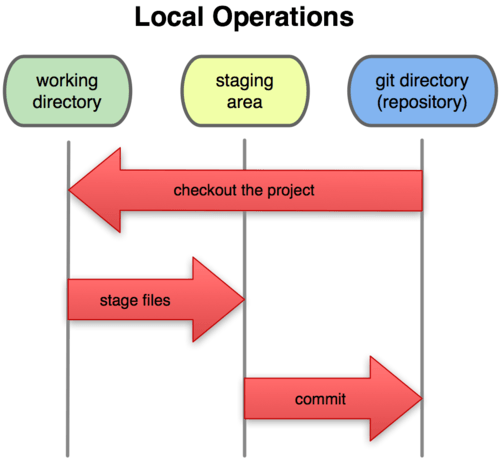
\includegraphics[width=.8\textwidth]{figs/sections.png}\cite{book}
    \end{center}
}

\subsection{Undoing}
\begin{frame}[fragile]
    \frametitle{Undoing Changes to Working Directory}

    \verb|$ git checkout <filename>|
    \begin{itemize}
        \item Put file from staging area into working directory
        \item Undo unstaged changes to file
    \end{itemize}
    \verb|$ git checkout <commit> -- <filename>|
    \begin{itemize}
        \item Put file from specified commit into working directory and
              staging area
        \item Overwrite unstaged changed to file
    \end{itemize}

    The \verb|checkout| command has other uses when dealing with branches
    (discussed later). Be warned -- \verb|git checkout <commit>| without
    filename argument does not do what you expect.
\end{frame}

\begin{frame}[fragile]
    \frametitle{Erasing Unstaged Changes}
    \begin{tcblisting}{listing only}
$ git checkout name_file.txt
$ cat name_file.txt 
Hi, my name is Andrew
I like git
    \end{tcblisting}
\end{frame}

% TODO Funny spacing
\begin{frame}[fragile]
    \frametitle{Undoing Changes to Staging Area}

    The \verb|reset| command is similar to \verb|checkout| for staging area

    \verb|$ git reset|
    \begin{itemize}
        \item Unstage all changes
        \item Reset staging area to HEAD
    \end{itemize}
    \verb|$ git reset <filename>|
    \begin{itemize}
        \item Unstage changes to file
        \item Reset file in staging area to HEAD
    \end{itemize}

    The \verb|reset| command will not touch the working directory unless
    passed an additional argument. Follow \verb|reset| with \verb|checkout|
    to undo changes to working directory.

    The \verb|reset| command, like \verb|checkout|, has other uses related
    to branches, but we will not cover these.
\end{frame}

\begin{frame}[fragile]
    \frametitle{Erasing Unstaged Changes}
    \begin{tcblisting}{listing only}
$ git reset name_file.txt
Unstaged changes after reset:
M	name_file.txt
$ git checkout name_file.txt
$ cat name_file.txt 
Hi, my name is Andrew
    \end{tcblisting}
\end{frame}

\subsection{Reviewing}
\begin{frame}[fragile]
    \frametitle{Viewing History}

    \verb|$ git log [<since>..<until>] [-- <path>]|
    \begin{itemize}
        \item Show commit logs
        \item \verb|$ git log HEAD~3..HEAD^|
        \item \verb|$ git log -- file-with-bug.c|
    \end{itemize}

    \verb|$ git show <object>|
    \begin{itemize}
        \item Show various types of objects
        \item \verb|$ git show HEAD@{yesterday}|
        \item \verb|$ git show HEAD:file|
    \end{itemize}
\end{frame}

\begin{frame}[fragile]
    \frametitle{Viewing Log}
    \begin{tcblisting}{listing only}
$ git log
commit 4f6f4a4a4d432a8c22fda5dff7006dfc026e126f
Author: Your Name <you@example.com>
Date:   Mon Apr 3 22:05:50 2017 -0500

    Add ignore file

commit dec6e96fe5ad9d2f419e775c2f4a1b0ac52316e2
Author: Your Name <you@example.com>
Date:   Mon Apr 3 17:37:57 2017 -0500

    Add greeting
    \end{tcblisting}
\end{frame}

\begin{frame}[fragile]
    \frametitle{Referencing Objects}

    \begin{itemize}
        \item \verb|a88dbbe57b9e9fc01f701c45c405647c588e6a6a|
        \item \verb|a88d|
        \item \verb|v1.0.3|
        \item \verb|master|
        \item \verb|origin/master|
        \item \verb|HEAD|
        \item \verb|HEAD^ == HEAD~1|
        \item \verb|feature_brach@{May.30}|
    \end{itemize}
\end{frame}

\begin{frame}[fragile]
    \frametitle{Examining Commit Object}
    \begin{tcblisting}{listing only}
$ git show dec6e
commit dec6e96fe5ad9d2f419e775c2f4a1b0ac52316e2
Author: Your Name <you@example.com>
Date:   Mon Apr 3 17:37:57 2017 -0500

    Add greeting

diff --git a/name_file.txt b/name_file.txt
new file mode 100644
index 0000000..c987f6b
--- /dev/null
+++ b/name_file.txt
@@ -0,0 +1 @@
+Hi, my name is Andrew
    \end{tcblisting}
\end{frame}

\begin{frame}[fragile]
    \frametitle{Log Formatting}

    \verb|$ git log --pretty=<format>|
    \begin{itemize}
        \item \verb|oneline|
        \item \verb|full|
        \item \verb|format:"hash: %h author: %an date: %ad"|
		\item see git-log(1) for more options
    \end{itemize}
	\verb|$ git log --graph --pretty=oneline|
\end{frame}

\begin{frame}[fragile]
    \frametitle{Using History}
    \begin{tcblisting}{listing only}
$ echo 'I like git' >> name_file.txt
$ echo 'Hello, world!' >> name_file.txt
$ git commit -am 'Share more information'
Share more information
 1 file changed, 2 insertions(+)
    \end{tcblisting}
\end{frame}

\begin{frame}[fragile]
    \frametitle{Using History}
    \begin{tcblisting}{listing only}
$ git diff HEAD~2
diff --git a/.gitignore b/.gitignore
new file mode 100644
index 0000000..d0833a3
--- /dev/null
+++ b/.gitignore
@@ -0,0 +1,2 @@
+*.out
+todo_list.txt
diff --git a/name_file.txt b/name_file.txt
index c987f6b..d5e2134 100644
--- a/name_file.txt
+++ b/name_file.txt
@@ -1 +1,3 @@
 Hi, my name is Andrew
+I like git
+Hello, world!
    \end{tcblisting}
\end{frame}

\begin{frame}[fragile]
    \frametitle{Using History}
    \begin{tcblisting}{listing only}
$ git show HEAD~1:name_file.txt 
Hi, my name is Andrew
$ git checkout HEAD~1 -- name_file.txt
    \end{tcblisting}
\end{frame}

\subsection{Branching}
\frame
{
    \frametitle{Three Branches}

	\begin{center}
		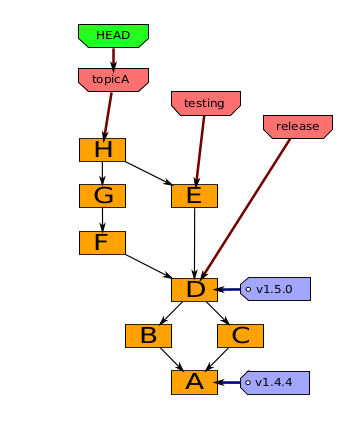
\includegraphics[height=.8\textheight]{figs/complicated-dag.png}
	\end{center}
}

\begin{frame}[fragile]
    \frametitle{Branching}

    \verb|$ git branch -l|
    \begin{itemize}
        \item List local branches
    \end{itemize}

    \verb|$ git branch <branchname> |
    \begin{itemize}
        \item Create new branch on HEAD
    \end{itemize}

    \verb|$ git branch <branchname> <start-commit>|
    \begin{itemize}
        \item Create new branch on specified commit
    \end{itemize}

    \verb|$ git checkout <branch>|
    \begin{itemize}
        \item Checkout branch by name
    \end{itemize}

    \verb|$ git checkout -b <branchname> [<start-commit>]|
    \begin{itemize}
        \item Create and switch to a new branch
    \end{itemize}
\end{frame}

\begin{frame}[fragile]
    \frametitle{Branch Example}
    \begin{tcblisting}{listing only}
$ echo 'var = 3' > math_file.py
$ git add math_file.py 
$ git commit -m 'Start programming'
[master af23d01] Start programming
 1 file changed, 1 insertion(+)
 create mode 100644 math_file.py
    \end{tcblisting}
\end{frame}

\frame
{
    \frametitle{Before Branch}

	\begin{center}
		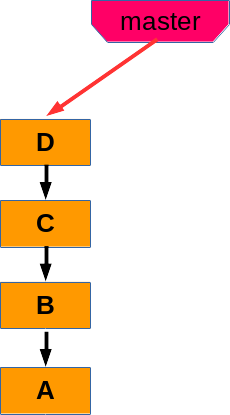
\includegraphics[height=.8\textheight]{figs/1-before-branch.png}
	\end{center}
}

\begin{frame}[fragile]
    \frametitle{Branch Example}
    \begin{tcblisting}{listing only}
$ rm *.out todo_list.txt
$ touch file1 file2 file3
$ git branch math
$ git checkout math
Switched to branch 'math'
$ git add .
$ git commit -m 'Add more files'
[math db71718] Add more files
 3 files changed, 0 insertions(+), 0 deletions(-)
 create mode 100644 file1
 create mode 100644 file2
 create mode 100644 file3
    \end{tcblisting}
\end{frame}

\frame
{
    \frametitle{First Branch Commit}

	\begin{center}
		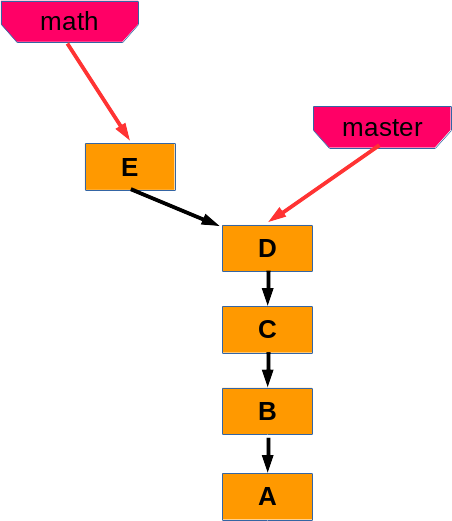
\includegraphics[height=.8\textheight]{figs/2-first-branch.png}
	\end{center}
}

\begin{frame}[fragile]
    \frametitle{Branch Example}
    \begin{tcblisting}{listing only}
$ ls
file1  file2  file3  math_file.py  name_file.txt
$ git checkout master
Switched to branch 'master'
$ ls
math_file.py  name_file.txt
    \end{tcblisting}
\end{frame}

\begin{frame}[fragile]
    \frametitle{Branch Example}
    \begin{tcblisting}{listing only}
$ echo 'x = 0.5 * var' >> math_file.py 
$ git commit -am 'Make change to master branch'
[master 7864aac] Make change to master branch
 1 file changed, 1 insertion(+)
$ git checkout math
Switched to branch 'math'
$ cat math_file.py 
var = 3
    \end{tcblisting}
\end{frame}

\frame
{
    \frametitle{Master Branch Commit}

	\begin{center}
		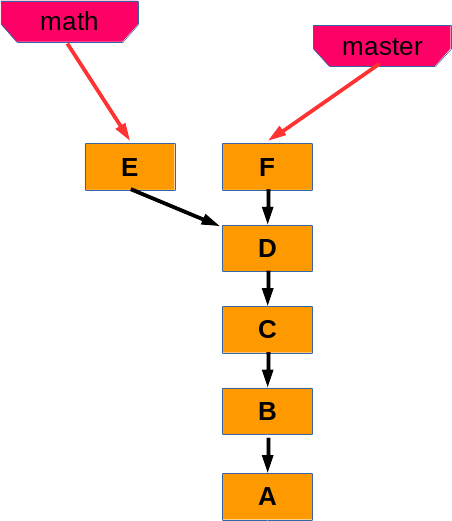
\includegraphics[height=.8\textheight]{figs/3-master-commit.png}
	\end{center}
}

\begin{frame}[fragile]
    \frametitle{Branch Example}
    \begin{tcblisting}{listing only}
$ cat math_file.py 
var = 3
$ echo ' x = 1/2. * var' >> math_file.py 
$ git commit -am 'Make conflicting change to math branch'
[math 6a015d3] Make conflicting change to math branch
 1 file changed, 1 insertion(+)
    \end{tcblisting}
\end{frame}

\frame
{
    \frametitle{Another Math Commit}

	\begin{center}
		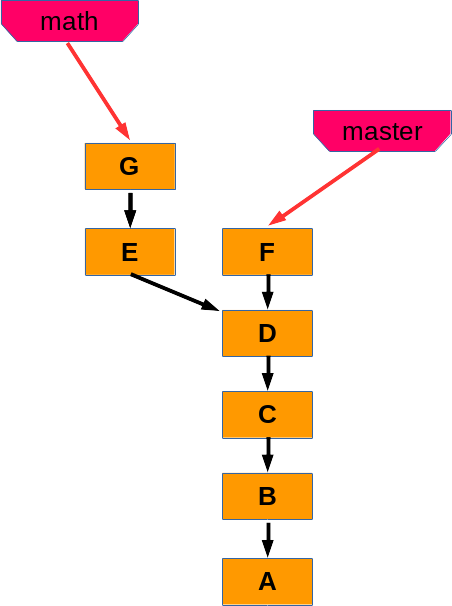
\includegraphics[height=.8\textheight]{figs/4-branch-commit.png}
	\end{center}
}

\begin{frame}[fragile]
    \frametitle{Merging}

    \verb|$ git merge <branch>|
    \begin{itemize}
        \item Incorporate changes from specified branch into current
            branch
        \item Conflicts may result
        \item Any conflicts must be resolved before merge is completed
    \end{itemize}
\end{frame}

\begin{frame}[fragile]
    \frametitle{Merge Example}
    \begin{tcblisting}{listing only}
$ git checkout master
Switched to branch 'master'
$ git merge math
Auto-merging math_file.py
CONFLICT (content): Merge conflict in math_file.py
Automatic merge failed; fix conflicts and then commit the result.
$ cat math_file.py 
var = 3
<<<<<<< HEAD
x = 0.5 * var
=======
 x = 1/2. * var
>>>>>>> math
    \end{tcblisting}
\end{frame}

\begin{frame}[fragile]
    \frametitle{Merge Example}
    \begin{tcblisting}{listing only}
... fix changes
$ git status
On branch master
You have unmerged paths.
  (fix conflicts and run "git commit")
  (use "git merge --abort" to abort the merge)

Changes to be committed:

	new file:   file1
	new file:   file2
	new file:   file3

Unmerged paths:
  (use "git add <file>..." to mark resolution)

	both modified:   math_file.py
    \end{tcblisting}
\end{frame}

\begin{frame}[fragile]
    \frametitle{Merge Example}
    \begin{tcblisting}{listing only}
$ git add math_file.py
$ git commit
[master 211a76d] Merge branch 'math'
$ ls
file1  file2  file3  math_file.py  name_file.txt
    \end{tcblisting}
\end{frame}

\frame
{
    \frametitle{After Merge}

	\begin{center}
		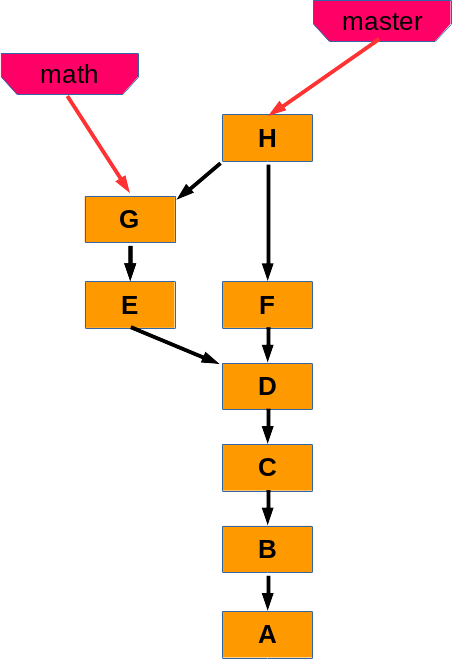
\includegraphics[height=.8\textheight]{figs/5-after-merge.png}
	\end{center}
}

\begin{frame}[fragile]
    \frametitle{Mergetool}

    \verb|$ git mergetool|
    \begin{itemize}
        \item Presents a visual interface to merging
        \item Example: \verb|$ git mergetool --tool=meld|
    \end{itemize}
    \begin{center}
        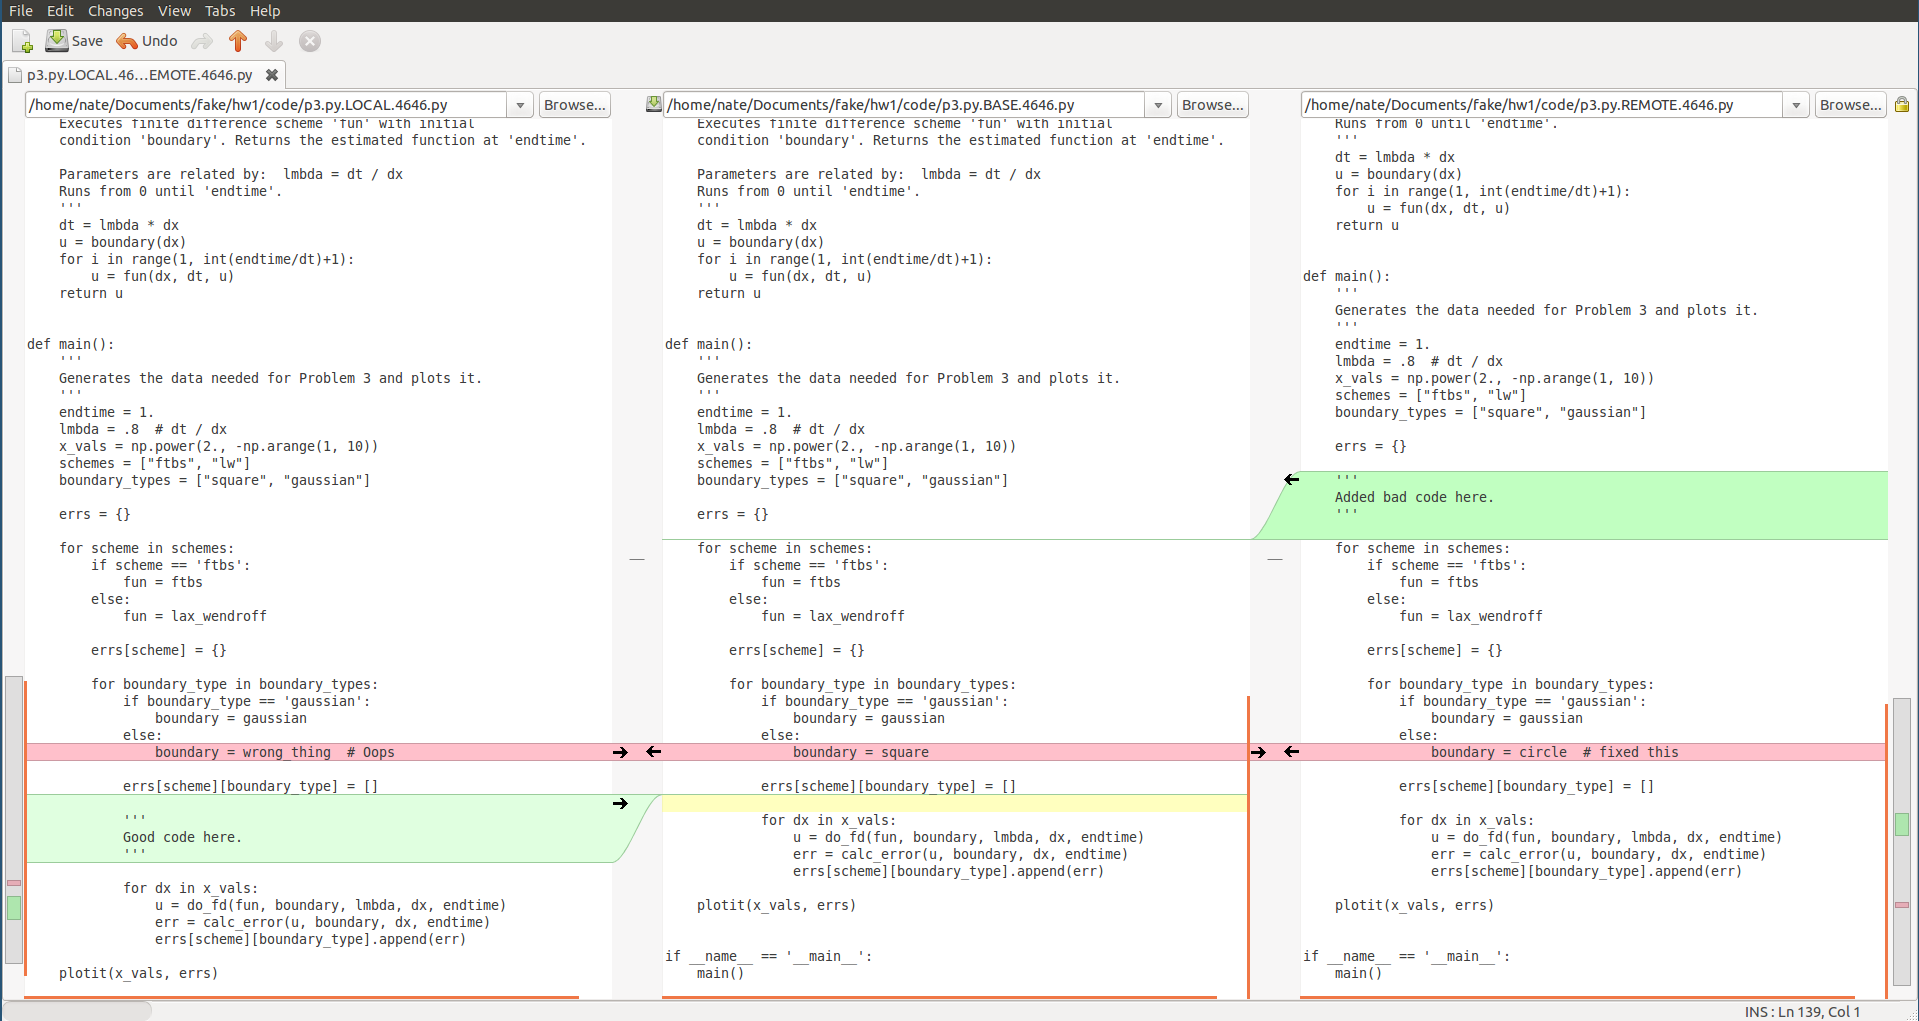
\includegraphics[width=.9\textwidth]{figs/meld-screenshot}
    \end{center}

\end{frame}

\subsection{Other Commands}
\begin{frame}[fragile]
    \frametitle{Changing Settings}

	\verb|$ git config --list|
	\begin{itemize}
		\item Lists the current configuration settings
	\end{itemize}
	\verb|$ git config <key>|
	\begin{itemize}
		\item Gets the current value of \verb|key|
	\end{itemize}
	\verb|$ git config [level] <key> <value>|
	\begin{itemize}
		\item Changes setting \verb|key| to \verb|value|
		\item Optional \verb|level| determines scope of setting
		\begin{itemize}
			\item Omitting \verb|level|: repository
			\item \verb|--global|: user
			\item \verb|--system|: system
		\end{itemize}
	\end{itemize}
\end{frame}

\begin{frame}[fragile]
    \frametitle{Common Configuration Settings}
	A few settings you will want to update when first using Git:\\ \ \\
	\verb|$ git config --global user.name "John Doe"|
	\verb|$ git config --global user.email johndoe@example.com|
	\verb|$ git config --global core.editor emacs|
	\verb|$ git config --global core.excludesfile ~/.gitignore|
	\verb|$ git config --global merge.tool meld|
\end{frame}

\begin{frame}[fragile]
    \frametitle{Getting Help}

	\verb|$ git help <command>|
	\begin{itemize}
		\item Display \textit{a lot} of information about command
	\end{itemize}

    Google and StackOverflow are great resources for quick questions.
    Chances are that almost any \verb|git| question you have has been
    asked and answered already.

\end{frame}

\section{Sharing}
\begin{frame}[fragile]
    \frametitle{Remotes Repository}
	\begin{center}
		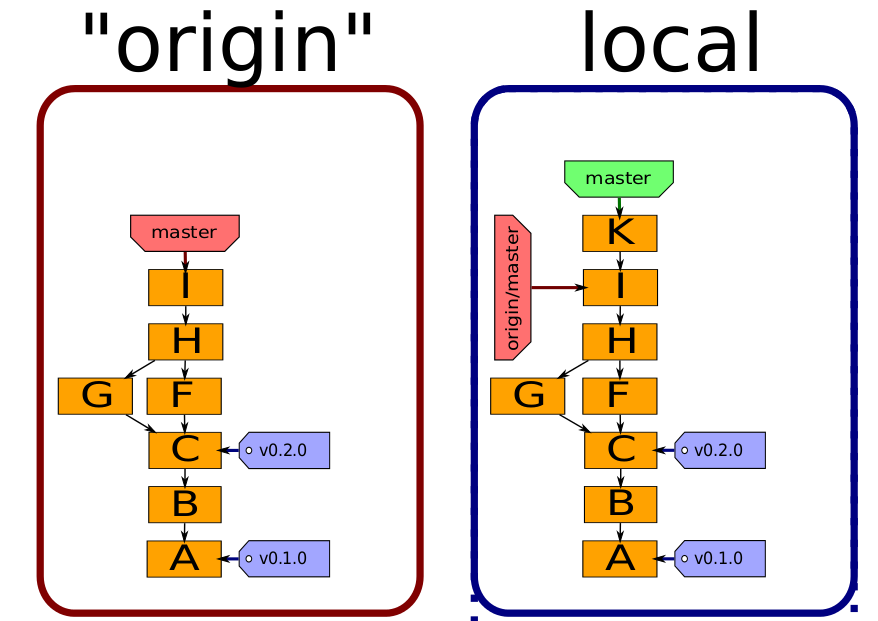
\includegraphics[width=.8\textwidth]{figs/single-remote}
	\end{center}
\end{frame}

\begin{frame}[fragile]
    \frametitle{Remotes}

    \verb|$ git remote add <name> <url>|
    \begin{itemize}
        \item Adds a remote named \verb|<name>| for the repository at \verb|<url>|
    \end{itemize}

    \verb|$ git branch -r |
    \begin{itemize}
        \item List remote branches
        \item Use \verb|$ git merge| to merge these branches
    \end{itemize}
\end{frame}

\begin{frame}[fragile]
    \frametitle{Remotes (2)}

    \verb|$ git fetch <remote>|
    \begin{itemize}
        \item Fetches updates from specified remote
        \item \verb|$ git fetch --all|
    \end{itemize}

    \verb|$ git pull [<remote>] [<branch>]|
    \begin{itemize}
        \item Short for a fetch followed by a merge
    \end{itemize}

    \verb|$ git push [<remote>] [<branch>]|
    \begin{itemize}
        \item Send updates to remote
        \item Similar to running \verb|pull| on remote machine
        \item No conflicts allowed
    \end{itemize}
\end{frame}

\begin{frame}[fragile]
    \frametitle{Git Naming--Disambiguation}
    Git creates branches automatically in certain cases.
    \begin{itemize}
        \item \verb|HEAD|: special reference that identifies the current branch
        \item \verb|master|: Default branch created when a repository is first 
            initialized
        \item \verb|origin|: default name chosen for a remote when cloned
        \item \verb|<remote_name>/<branch_name>|
            \begin{itemize}
                \item \verb|origin/master|
                \item \verb|upstream/fix-issue-105|
            \end{itemize}
    \end{itemize}
\end{frame}

\begin{frame}[fragile]
    \frametitle{Remotes Example}
	``fred'' cannot push to ``origin''

	\begin{center}
		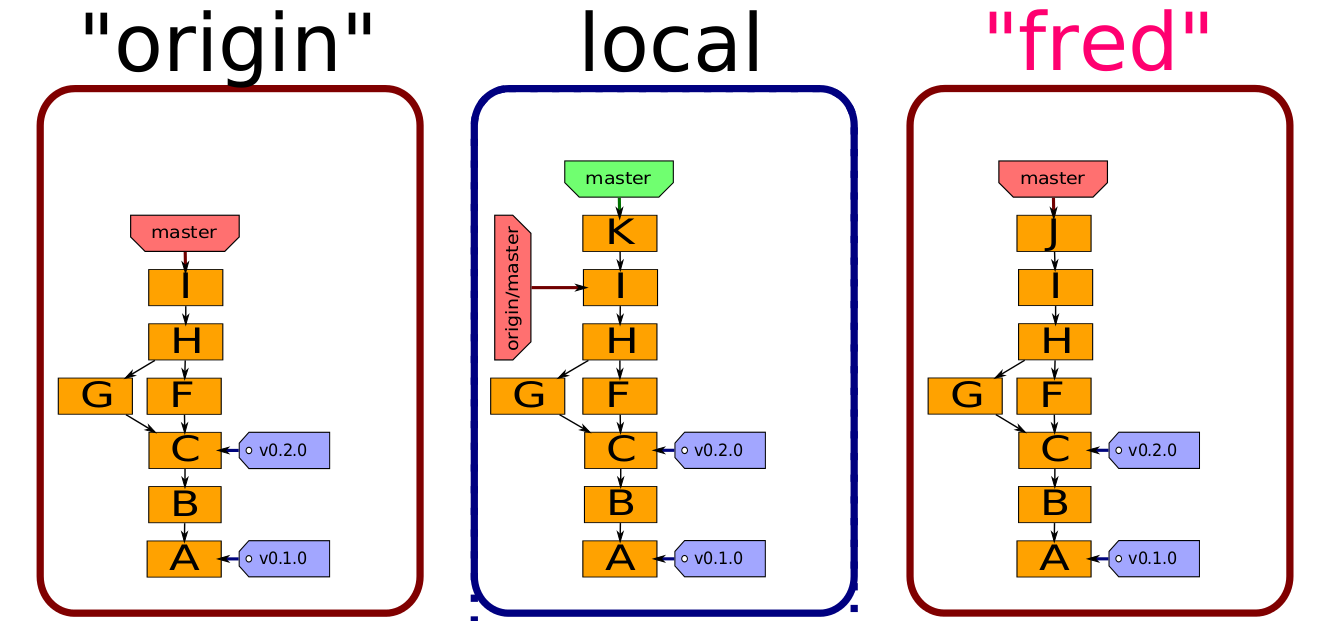
\includegraphics[width=.8\textwidth]{figs/several-remotes}
	\end{center}
\end{frame}

\begin{frame}[fragile]
    \frametitle{Remotes Example (continued)}
	Fetch from ``fred''

	\begin{center}
		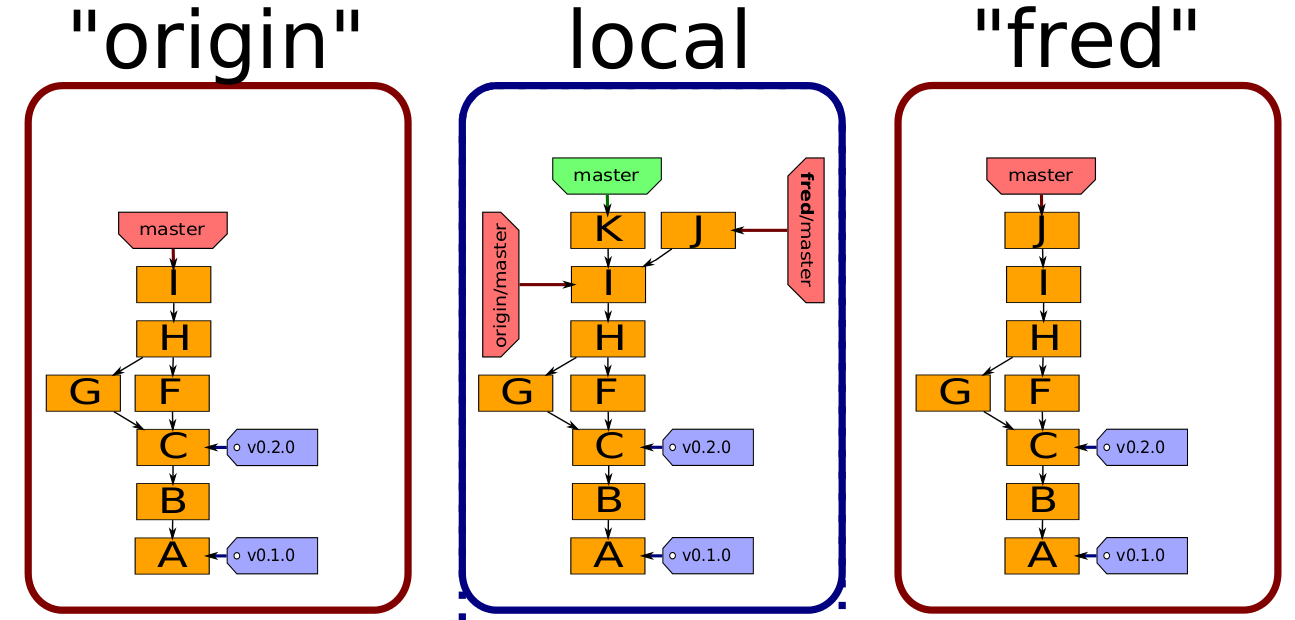
\includegraphics[width=.8\textwidth]{figs/fetch-fred}
	\end{center}
\end{frame}

\begin{frame}[fragile]
    \frametitle{Remotes Example (continued)}
	Merge in the changes

	\begin{center}
		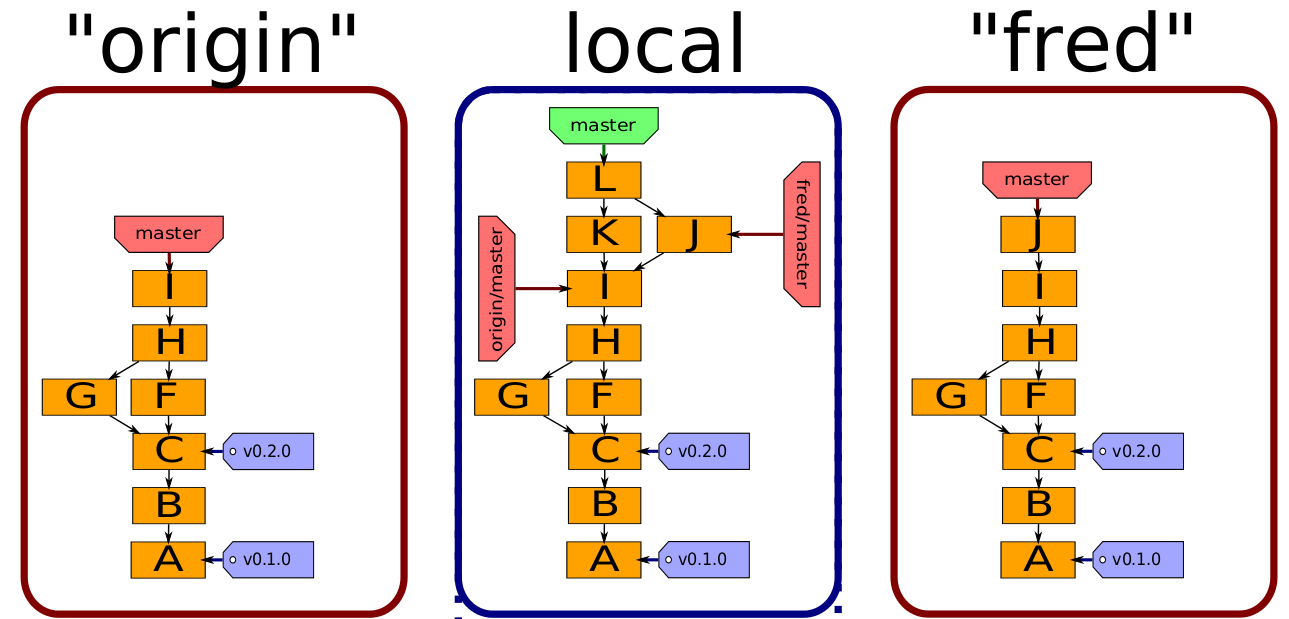
\includegraphics[width=.8\textwidth]{figs/merge-fred}
	\end{center}
\end{frame}

\begin{frame}[fragile]
    \frametitle{Remotes Example (continued)}
	Push changes to ``origin''

	\begin{center}
		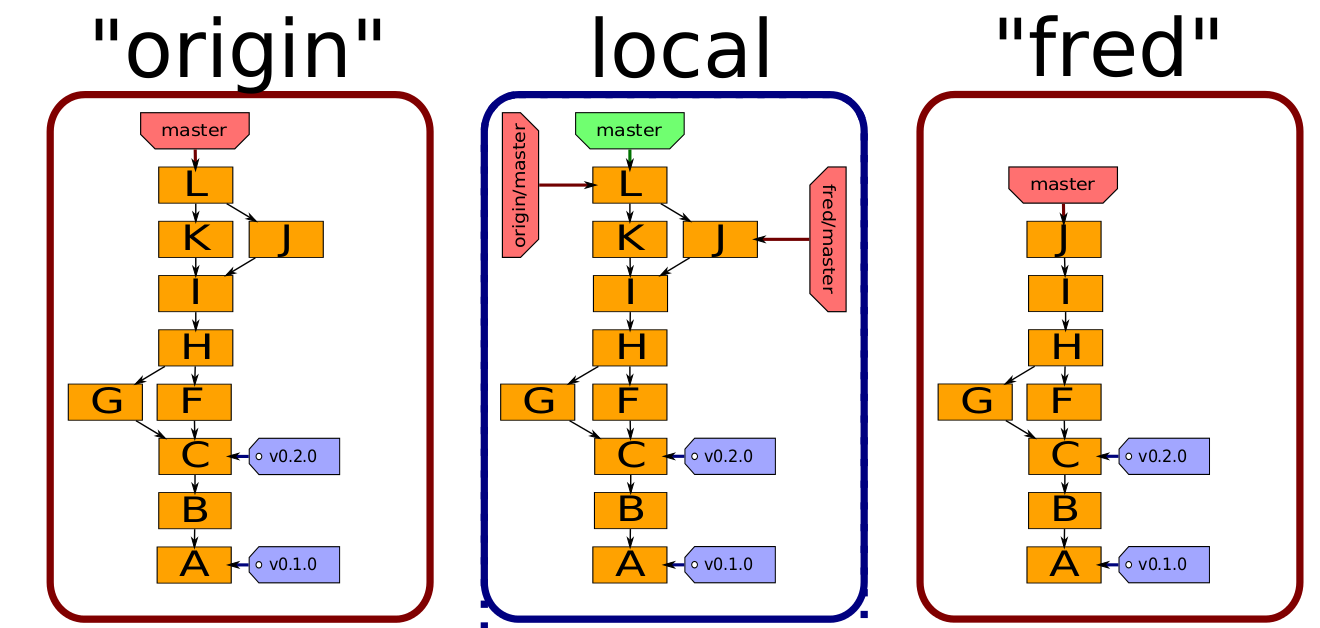
\includegraphics[width=.8\textwidth]{figs/push-fred}
	\end{center}
\end{frame}

\begin{frame}[fragile]
    \frametitle{Challenge Problem}

    Shape module at \verb|https://github.com/gswg/example.git|
    \begin{itemize}
        \item Clone repository
        \item Locate and fix bug
        \item Push fix
            \begin{itemize}
                \item You may need to fetch and merge with \verb|origin/master|
                \item Username: gswg
                \item Password: siam2014
            \end{itemize}
    \end{itemize}
\end{frame}

\frame
{
    \frametitle{Distributed}
    \begin{itemize}
        \item No central location that keeps track of your data (no single place is more important than another)
        \item Encourages small commits and frequent merging
        \item Branches don't affect the main repository and can commit changes without disturbing others
        \item Work offline
        \item Rely on a network of trust
    \end{itemize}
}

\subsection{Distributed Workflows}
\frame
{
    \frametitle{Centralized Workflow}

    \begin{center}
        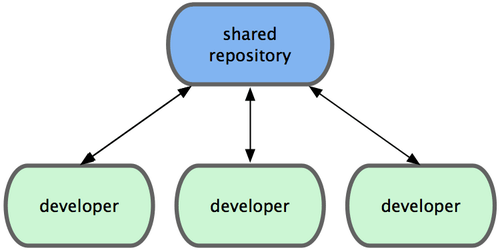
\includegraphics[width=.7\textwidth]{figs/centralized-workflow.png}\cite{book}
    \end{center}
}

\frame
{
    \frametitle{Integration-Manager Workflow}

    \begin{center}
        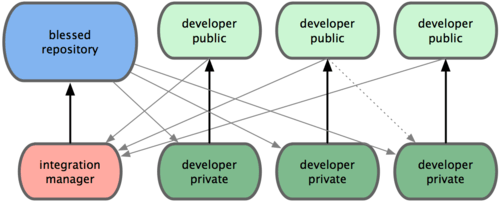
\includegraphics[width=.7\textwidth]{figs/integration-manager-workflow.png}\cite{book}
    \end{center}

}

\frame
{
    \frametitle{Dictator and Lieutenants Workflow}

    \begin{center}
        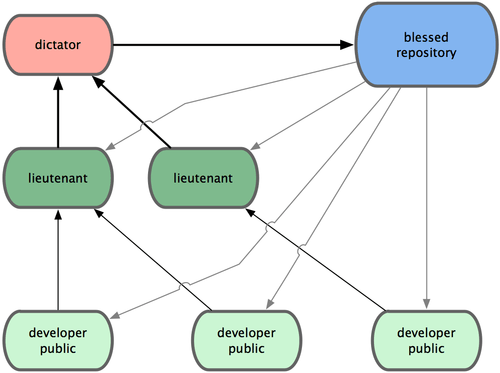
\includegraphics[width=.7\textwidth]{figs/dictator-lieutenant-workflow.png}\cite{book}
    \end{center}

}

\frame
{
    \frametitle{Free and Open Source}

    \begin{itemize}
        \item Downloads at \url{http://git-scm.com}
        \item Libgit2: free and open source library for writing custom Git applications
        \begin{columns}
            \begin{column}{.5\textwidth}
                \begin{center}
                    
\includegraphics[width=1\textwidth]{figs/git-logo1.png}
                \end{center}
            \end{column}
            \begin{column}{.5\textwidth}
                \begin{center}
                    
\includegraphics[width=1\textwidth]{figs/libgit-logo.png}
                \end{center}
            \end{column}
        \end{columns}
    \end{itemize}
}

\subsection{Git on the Web}
\frame
{
    \frametitle{GitHub}

    \begin{itemize}
        \item Powerful web interface for publishing Git repositories
        \item Simple to view changes and track progress on repositories
        \item Wiki and bug tracking built into each repository 
    \end{itemize}
    
    \begin{center}
        
\includegraphics[width=.8\textwidth]{figs/github-logo.png}
    \end{center}
}

\frame
{
    \frametitle{Bitbucket}

    \begin{itemize}
        \item Similar to GitHub
        \item Allows private repositories for students
    \end{itemize}
    
    \begin{center}
        
\includegraphics[width=.8\textwidth]{figs/bitbucket-logo.png}
    \end{center}
}

\frame
{
\small
    \frametitle{References}
    \renewcommand{\section}[2]{}
    \bibliographystyle{plainnat}
    \bibliography{git_slides}
}
\end{document}
